% NOTES ONLY, to be written. Trimmed 2026-11-07 from thesis/methodology/05_features.tex and
% 05a-05d (full drafts in git, commit e4eb857). Figures still in thesis/methodology/:
% features_overview_schematic.{py,pdf} and turning_feature_schematic.{py,pdf}.
% CHECK: CGPS_data/thesis_final/ holds only turning_feature.py and split_check.py; taper, angle and
% ratios have no final script yet, so their text cannot be written to the code yet.
%
% Umbrella section should contain:
% - Features drawn from studies relating geometry to low WSS or plaque location (ch:literature,
%   sec:method-selection), some adapted (curvature on 3D centerlines over a fixed chord).
% - Read from the arteries of sec:method-split, points in mm with an artery label, traversed from
%   the ostium. Open: in split_trunks.py the LAD and LCx paths start at the LM bifurcation, not at
%   the ostium; only the RCA starts at the ostium.
% - Curvature and taper per segment; angle and ratios once per participant at the LM bifurcation.
%   Open: the split points carry no lumen radius, and the tracer gives a contour per step, not a mask.
% - Table tab:method-features (feature, measured on, input, section) and the overview figure
%   fig:method-features.
% - Shared rules: unit of measurement; missing values (TODO).
\section{Geometric Features}
\label{sec:method-features}

\todonote{To be written: where the features come from, what they are read from, and the overview table and figure.}

% NOTES ONLY, to be written. Trimmed 2026-11-07 from thesis/methodology/05a_curvature.tex
% (full draft in git, commit e4eb857). Implementation: CGPS_data/thesis_final/turning_feature.py
% (mean_turning, segment_turning) on each artery from split_trunks.py; figure from
% turning_feature_schematic.py.
%
% The subsection should contain:
% - Curvature as mean turning angle per mm, a form of average curvature, the tortuosity measure most
%   closely, although weakly, related to low WSS (kashyap2022tortuosity; simulation study, keep
%   "although weakly").
% - Turning angle at each point between two 5 mm chords, chord ends by linear interpolation;
%   atan2 form (eq:method-turn), unsigned in [0, pi].
% - Noise: a positional error sigma gives spurious turning that falls with the square of the chord
%   length; 5 mm chord as in vanzandwijk2019curvature. No further smoothing; no values within 5 mm of
%   either artery end. TODO: confirm with Kit that the tracer centerlines arrive smoothed.
% - Profile kappa = theta / l in rad/mm (eq:method-profile, referred to by curvature_fpca), computed
%   on the whole artery and then divided at the segment boundaries.
% - Segment value T_s = arc-length mean of the profile (eq:method-tl), trapezoid rule; fewer than two
%   profile points -> missing.
% - Difference from Tello Ayala et al. (2D, consecutive points): 3D, fixed chord, normalised by
%   length, so independent of point spacing.
% - Figure fig:method-turning.
\subsection{Turning-angle curvature}
\label{sec:method-curvature}

\todonote{To be written: turning angle over 5\,mm chords, the curvature profile and its arc-length mean per segment.}

% Methods, subsection of sec:method-features: the bifurcation angle only. Which segments it enters
% (proximal LAD and LCx) and why belong to 05_features.tex, how it enters the model to
% sec:method-models.
% Implementation (since 2026-11-10): CGPS_data/thesis_final/bifurcation_angle.py (point_at_depth,
% angle_between, lm_angle, tree_angle; DEPTHS = 5 to 10 mm in 0.5 mm steps) on the LAD and LCx
% arteries of split_trunks.split. Replaces who_where_readiness.lm_bifurcation_angle (Medis labels,
% centroid of points 2 to 8 mm, one bifurcation point per daughter; no published source).
% Source: Medrano-Gracia et al. 2016 (medranogracia2016atlas), read in full 2026-11-10: "A bifurcation
%   point was automatically calculated from the centrelines at the point where the centrelines split";
%   measurements "at a range of depths from this bifurcation point in 0.5 mm steps, following the
%   centrelines" (arc length); angle B "the angle of the bifurcation between the distal main vessel
%   and the side branch" (for the LM: LAD to LCx); "Computationally, these angles have to be defined
%   with linear approximations of the centrelines"; reported "as the average in the 5-10 mm depth
%   interval"; "averaging angles in the 5-10 mm interval ensures a more robust measurement than a
%   single point" (word "robust" is theirs, not used here); the angle "slowly decreases as the
%   measurement is taken further from the bifurcation point". Their values: 78.9 +- 23.1 deg (N = 300),
%   89 deg with and 75 deg without an intermediate artery.
% CHECK: how the "linear approximations" were fitted is not stated. The code uses the line from the
%   bifurcation point to the centerline point at each depth; keep "follows", never "replicates".
% CHECK: the bifurcation point is the first point shared by the tracer LAD and LCx
%   (split_trunks.split starts both there when their paths share a node; otherwise the paths start after
%   a labelled LM, the points differ and the angle is missing). How often this happens in the tracer
%   trees is unknown until they are run.
% OPEN: ramus intermedius. The tracer labels only the artery, so a ramus is not separated; the atlas
%   found the angle 14 deg wider with one. Handling belongs to sec:method-validity-definitions.
% CAREFUL: progression_who_pooled.py still takes the angle from the old Medis function, so the model
%   and this text disagree until that script calls tree_angle.
% Not used: angle A or C, the inflow angle (their own definitions, not in the five features), 2D
%   projection (EBC: 3D is needed). Not stated in the text (counterfactual rule).
% 2026-11-10 (user: Aida methodology guide over sec:method-angle; no "The feature chosen", no
%   First/Finally). Facts, cite, label and eq:method-angle unchanged. Changed: opener chains to the
%   division into segments and names the input (guide 4.1); equation chain with a where sentence naming
%   every symbol and one sentence on what theta tells (9.1); the mean over depths is now an equation,
%   eq:method-angle-mean (9.1); the depth interval as concede-and-defend with its cost named (5); step
%   markers removed, each step opens with what is measured. Cut: "since the tracer labels only the
%   artery ..." (a reason about the tracer's design that was not checked against the labels).
\subsection{Bifurcation Angle}
\label{sec:method-angle}

Note: Research if this is better to have two angles going into the model proximal main vessel and the side branch, and angle the angle between the proximal and distal main vessel. Also research if the inflow angle is important and should be included.

 
The bifurcation point $O$ was taken as the first centerline point shared by the LAD and the LCx, where their arc length starts.
At the arc length $d$ from $O$, the points $L(d)$ on the LAD and $C(d)$ on the LCx were found, and the angle between the lines from $O$ to these points was computed as
\begin{equation}
  \theta(d) = \operatorname{atan2}\!\left( \lVert (L(d) - O) \times (C(d) - O) \rVert ,\; (L(d) - O) \cdot (C(d) - O) \right) ,
  \label{eq:method-angle}
\end{equation}
where $\times$ and $\cdot$ denote the cross product and the dot product of two vectors, $\lVert \cdot \rVert$ the length of a vector, and $\operatorname{atan2}$ the angle that has this cross-product length and this dot product.
$\theta(d)$ lies between 0 and 180 degrees, and a wider angle means that the two arteries leave the bifurcation further apart.

The bifurcation angle $\bar\theta$ was the mean over the depths from 5 to 10\,mm in steps of 0.5\,mm:
\begin{equation}
  \bar\theta = \frac{1}{11} \sum_{d \in \{5,\,5.5,\,\ldots,\,10\}} \theta(d) ,
  \label{eq:method-angle-mean}
\end{equation}
where the eleven depths are in mm along the arteries from $O$.
Although the angle depends on the depth at which it is measured, this interval follows Medrano-Gracia et al., who used it because the angle decreases slowly with depth, and averaging over it keeps $\bar\theta$ from resting on one depth.
The cost is that bends in the first 10\,mm of the arteries enter the angle.
$\bar\theta$ was recorded as missing for participants whose LAD and LCx share no first point or whose LAD or LCx is shorter than 10\,mm.

% Methods, subsection of sec:method-features: the two diameter-ratio features only. Why the bifurcation
% is represented at all belongs to sec:method-features and sec:lit-wss; which segment rows they enter
% (proximal LAD and LCx) to 05_features.tex and sec:method-models.
% 2026-11-11: written from daugther_ration_plan.md (same folder). Replaces the notes trimmed 2026-11-07
% (full draft in git, commit e4eb857).
% Decision (with the user, 2026-11-11): two features, still 2 parameters: daughter asymmetry
%   ln(D_LCx / D_LAD) and Finet's ratio D_LM / (D_LAD + D_LCx). Angle and the two ratios keep their own
%   linear terms in the tested geometry block (5 parameters); angle x asymmetry is one prespecified
%   secondary term, estimated, outside the LR test (one simulation study on synthetic trees, and a
%   product needs its main effects). Owned by sec:method-models.
% Rejected, not stated in the text (counterfactual rule): the LM->LAD and LM->LCx ratios planned
%   before 2026-11-11. Both divide by the LM diameter, the least reliable of the three (LM length
%   10.5 +- 5.3 mm in Medrano-Gracia 2016, so the stretch clear of the ostium and of the confluence is
%   short or absent); its error enters both and correlates them, and both go missing together. The
%   review supports the LAD-LCx width difference (Garcha 2025) and discusses Finet's ratio (Zhang 2024,
%   null); neither used LM->daughter ratios.
% Murray's exponent 3, the pooled 2.39 (taylor2024murray) and 7/3 (huo2012scaling) are no longer
%   needed here; the fact-ownership line for them in the content map (Thesis_coronary/CLAUDE.md) lapses.
% Implementation: CGPS_data/thesis_final/daughter_ratio.py (contour_area, contour_diameter,
%   reference_diameter, lm_ratios, tree_ratios; DEPTHS = (5, 10) mm, the interval of
%   bifurcation_angle.DEPTHS). Checked against the text line by line 2026-11-11: window 5 to 10 mm
%   from O, upstream for the LM; median over the points in the window; nan when the vessel does not
%   reach 10 mm or fewer than 2 points have a diameter there; no shared O -> both nan; short LM ->
%   Finet nan, asymmetry kept. Not in the text: the 3D polygon area (cross products about the centroid).
% Figure: content/methodology/figures/daughter_ratio_figure.py (made-up bifurcation, run through the
%   same code).
% Sources: medranogracia2016atlas ("effective radius", A = pi R^2, read 2026-11-10 for 05b);
%   finet2008fractal (0.678 as the reported mean of D_mother / (D_d1 + D_d2)).
% CHECK: Garcha full text not read (Nature redirect); abstract: "diameter ratio between left coronary
%   branches ... can amplify the effect of ... bifurcation angle". Its exact ratio definition and
%   direction are unverified, so the secondary term is not described as a replication.
% CHECK: 0.678 taken from the plan, not reread in Finet et al. this session. The plan's arithmetic
%   "3.39 / (2.708 + 2.236)" gives 0.686, not 0.678 (a ratio of means is not a mean of ratios); the
%   code check uses tubes of 3.39, 2.75 and 2.25 mm instead.
% CHECK: tracer contour format unknown (daughter_ratio.tracer_rings raises), so "the tracer's lumen
%   contour at each centerline point" is an assumption until the files are seen.
% (2026-11-13: the earlier CHECK on a 5 to 10 mm LM window is void; the LM window is the first 2 mm
%   from the ostium, see the 2026-11-11 entries below. Current definition: D = median area-equivalent
%   diameter, LAD/LCx 5 to 10 mm from O, LM 0 to 2 mm from the ostium; a = ln(D_LCx/D_LAD),
%   F = D_LM/(D_LAD + D_LCx). Report the coverage of F once the tracer LM lengths are known.)
% CAREFUL: progression_who_pooled.py has no ratios yet, so the model and this text disagree until it
%   calls tree_ratios.
% Style: prose only, British spelling, reason before method, no "trunk", no sentence opening "Because".
% 2026-11-11 (user: no First/Subsequently/Finally for short methods, true to the code but not every
%   detail, flow between sentences, A++ thesis voice). Body rewritten as connected prose; facts, labels,
%   cites and equations unchanged. Each step now follows from the one before (contour -> diameter ->
%   one diameter per vessel -> the two ratios -> missing rules). The stretch and median reasons merged
%   into one sentence after the method; "The cost is that a left main shorter than 10 mm has no
%   diameter" folded into the missing sentence. "A vessel with fewer than two contours counted as too
%   short" now stated as its effect (both ratios missing for a daughter, Finet only for the LM), as in
%   lm_ratios. Caption unchanged.
% 2026-11-11 (user: concise, only what fits a methodology section, as for 05b). Cut: "so D is the
%   diameter of the circle with the same area" ("area-equivalent" says it), the reading of a (0 for equal
%   daughters, negative when the LCx is narrower) and of F ("compares the left main with its two daughters
%   together", "a lower value means daughters that are wide for their parent"), and Finet's reported mean
%   0.678 (reference value, belongs in Results/Discussion when CGPS values are compared). Both features
%   now in one sentence with Figure B; "the same stretch as for the bifurcation angle" moved from the
%   opener to the stretch sentence; the LM-uncertainty reason joined into one sentence.
% 2026-11-11 (user: add a citation for the method): medranogracia2017bifurcation added as prior use of
%   Finet's ratio on CTA (read 2026-11-11, PMC5323506: D_PMV / (D_DMV + D_SB), 446 bifurcations in 211
%   normal CTAs, mean 0.6576 +- 0.083; the value is kept for Results/Discussion, as 0.678). CAREFUL: its
%   Methods do not say how the diameters were measured (lumen meshes cut by a 10 mm sphere at the
%   bifurcation point only), so cite it for the ratio on CTA, never for the diameter or the window. No
%   source found for the 5 to 10 mm diameter window or the median; both stay the thesis's own choices.
% 2026-11-11 (user: where is the LM diameter measured?): the stretch sentence split in two, LAD/LCx
%   downstream of O, LM upstream between O and the ostium. Checked medranogracia2016atlas (Computation
%   of Diameters, read 2026-11-11): effective diameter "every 0.5 mm from the ostium or previous main
%   bifurcation", i.e. the LM profile runs downstream from the ostium (Fig. 6A "Left main from ostia
%   (continuing to LAD)"), daughters from the bifurcation; LM reported at the ostium (3.7 mm, Results;
%   abstract 3.5 +- 0.8 mm, unexplained). No interval averaging for diameters (5 to 10 mm is for angles
%   only), and the positions behind their Finet's ratio are not stated. So the LM window upstream of O is
%   this thesis's choice, not theirs; never write "following" for it.
% 2026-11-11 (user: measure the LM at the ostium like the atlas; median over the first 2 mm, stated as a
%   design choice extending the atlas). Code: daughter_ratio.LM_OSTIUM = (0, 2) mm from the ostium, the
%   LM path no longer reversed; check() and the synthetic split_trunks tree confirm the window sits at the
%   ostium end. Missing rule now LM < 2 mm or < 2 contours there. Supersedes the 5 to 10 mm upstream
%   window and its CHECK above. The atlas Results give 3.7 mm at the ostium (abstract 3.5 +- 0.8 mm).
% CHECK: with an LM under about 4 mm the 2 mm window touches the confluence at O; and the number of
%   contours in 2 mm depends on the tracer point spacing (unknown). Report both once the tracer runs.
% CHECK: "where the lumen leaves the aorta" assumes the tracer's first LM contour sits at the aortic
%   junction; confirm on the tracer output.
% 2026-11-11 (user: add and cite Gharleghi 2025): gharleghi2025sex (IEEE TBME 72(7), 2025; read as
%   arXiv 2311.18489, 2.3): "The median diameter for each vessel, corresponding to the diameter of a
%   circle with equivalent cross-sectional area, was calculated over the 10mm segment" of each branch
%   within 10 mm arc length of the bifurcation point; Finet 0.57 in both sexes. "Adapted", not
%   "following": their stretch is 0 to 10 mm from the bifurcation point for all three vessels, ours 5 to
%   10 mm for the daughters and 0 to 2 mm from the ostium for the LM. Their reason for the median
%   (diameter changes little along 10 mm, SD 0.1 mm) differs from ours (side-branch origins).
% CHECK: bib entry from the arXiv author list and the journal citation found by search; pages and the
%   published author list not checked against IEEE Xplore.
% 2026-11-13 (user): Finet's ratio DROPPED as a model feature. Reasons (counterfactual rule, not in the
%   text): the review's only evidence is Zhang 2024's null; no sourced reason for a link to plaque
%   (Schoenenberger 2012, Murray deviation vs calcification, abstract only, cross-sectional); it is the
%   only feature needing the LM diameter, the least certain of the three, and it goes missing for a short
%   LM. Geometry block now 4 parameters (+1 secondary angle x asymmetry). The LM window, eq:method-finet,
%   finet2008fractal and medranogracia2017bifurcation are out of the text; the notes above on them are
%   history. daughter_ratio.py still returns "finet" (descriptive only, not in the model).
\subsection{Daughter Asymmetry}
\label{sec:method-ratio}

How the lumen is shared between the two branches at the left main bifurcation was described by the daughter asymmetry (Figure~\ref{fig:method-ratio}).

The tracer gives a lumen contour at each centerline point.
As the contours are rarely circular, each was reduced to its area-equivalent diameter, following Medrano-Gracia et al.\ \cite{medranogracia2016atlas},
\begin{equation}
  D = 2 \sqrt{A / \pi} ,
  \label{eq:method-diameter}
\end{equation}
where $A$ is the area enclosed by the contour (Figure~\ref{fig:method-ratio}A).
Each vessel was then given one diameter, the median of $D$ over a fixed stretch of its centerline, adapted from Gharleghi et al.\ \cite{gharleghi2025sex}, and the median keeps a single cross-section widened by a side-branch origin from moving the value.
For the LAD and the LCx the stretch was 5 to 10\,mm downstream of the bifurcation point $O$, the same stretch as for the bifurcation angle, which leaves out the widened lumen where the vessels join.

From the two diameters (Figure~\ref{fig:method-ratio}B), the daughter asymmetry
\begin{equation}
  a = \ln \frac{D_{\mathrm{LCx}}}{D_{\mathrm{LAD}}}
  \label{eq:method-asymmetry}
\end{equation}
was computed.

The asymmetry was missing whenever the angle was, or when the LAD or the LCx had fewer than two contours in its stretch.
A prespecified interaction between the angle and the asymmetry is described in Section~\ref{sec:method-models}.

\begin{figure}[htbp]
  \centering
  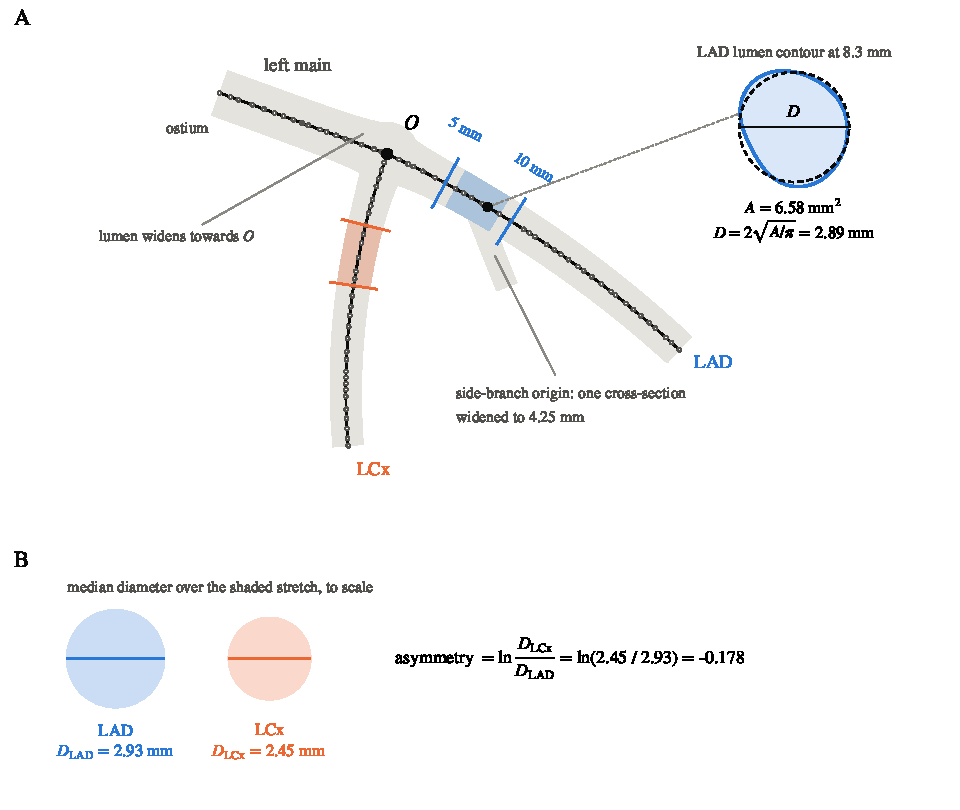
\includegraphics[width=\textwidth]{content/methodology/figures/daughter_ratio_figure.pdf}
  \caption{Daughter asymmetry on a made-up left main bifurcation, computed with the thesis code. Each lumen contour is reduced to the diameter $D$ of the circle with the same area, and the LAD and the LCx each to the median of $D$ over the shaded stretch 5 to 10\,mm from the bifurcation point $O$, which leaves out the widened lumen near $O$ and is not moved by the one cross-section widened at a side-branch origin (A). The two diameters, drawn to scale, give the daughter asymmetry (B).}
  \label{fig:method-ratio}
\end{figure}

% NOTES ONLY, to be written. Trimmed 2026-11-07 from thesis/methodology/05d_taper.tex
% (full draft in git, commit e4eb857). Implementation: tortuosity/taper.py, not yet in
% CGPS_data/thesis_final/.
%
% The subsection should contain:
% - Rationale: steady-flow WSS = 4 mu Q / (pi r^3) (malek1999shear); flow falls along the artery
%   with side branches, and with the pooled exponent 2.39 (taylor2024murray) taper carries only part
%   of the signal. Evidence for taper is thin (sec:lit-wss), no study links it to later plaque.
%   Log-radius slope is independent of overall calibre. Expected sign: lower taper -> lower WSS ->
%   more plaque, but sub-detection wall thickening could give the opposite sign. Open: two-sided
%   or signed test.
% - Size of the effect: about 0.25 mm diameter per 10 mm in normal arteries (medranogracia2016atlas),
%   about one voxel over 30 mm, so a robust fit over many cross-sections.
% - Computation in taper.py: resample every 0.5 mm; tangent from points 2.5 mm before and after;
%   orthogonal cut on a 12 x 12 mm grid at 0.1 mm, trilinear mask, threshold 0.5; area of the
%   connected region containing the centerline point; area-equivalent radius r = sqrt(A/pi)
%   (distance-transform radius kept for sensitivity). Open: how a voxel mask is formed from the
%   tracer's lumen contours.
% - Exclusions: first 3 mm, within two median radii of a side-branch junction, centerline point
%   outside the lumen, region touching the grid edge or another labelled vessel.
% - T = -10 b, b the Theil-Sen slope of ln r against s: fractional loss of radius per 10 mm.
%   Missing when remaining samples span < 20 mm or are < 60% of all samples.
% - Open: taper.py gives one T per artery, sec:method-selection uses taper per segment.
\subsection{Lumen Taper}
\label{sec:method-taper}

\todonote{To be written: rationale for taper and its Theil--Sen estimate from the lumen cross-sections.}

